\documentclass[../../statistical_learning_notes.tex]{subfiles}
\begin{document}
%%%%%%%%%%%%%%%%%%%%%%%%%%%%%%%%%%%%%%%%%%%%%%%%%%%%%%%%%%%%%%%%%%%%%%%%%%%
\section{Gaussian Process}
Suppose we have a set $X = (x_{1}, \ldots, x_{N}), x_{i} \in \mathbb{R}^{d}$. Then a random process $f(x)$ is a gaussian process if for any $n \leq N$, the joint distribution of any subset of size $n$ is a multivariate gaussian.
\begin{align*}
    \begin{bmatrix} f(x_{1})\\ f(x_{2})\\ \vdots\\ f(x_{n}) \end{bmatrix} \sim \mathcal{N} \bigg( \begin{bmatrix} m(x_{1})\\ m(x_{2})\\ \vdots\\ m(x_{n}) \end{bmatrix}, \begin{bmatrix} K(x_{1}, x_{1}) &\cdots &K(x_{1}, x_{n})\\ K(x_{2}, x_{1}) &\cdots &K(x_{2}, x_{n})\\ \vdots &\vdots &\vdots\\ K(x_{n}, x_{1}) &K(x_{n}, x_{2}) &\cdots &K(x_{n}, x_{n}) \end{bmatrix}  \bigg)\\
    K(x_{i}, x_{j}) = \hat{K}(x_{i} - x_{j}) \quad m(x) = constant \quad \text{for stationarity}
\end{align*}

where $m$ denotes the mean, and the matrix of kernels $K$ is a covariance matrix. Stationarity for a random process requires that the expected value be constant throughout and the variance between two points only be a function of their relative distance and not the position. Thus, a natural choice is to have the kernel as a function of the difference of $x_{i}$s. Several types of kernels satisfy this property
\begin{align*}
    \text{Radial Basis Function (RBF)} &= \sigma^{2}exp \bigg( -\frac{(x_{1} - x_{2})^{2}}{2l^{2}} \bigg) \; l = \text{length scale}\\
    \text{Rational Quadratic} &= \sigma^{2}\bigg(1 +\frac{(x_{1} - x_{2})^{2}}{2\alpha l^{2}} \bigg)^{-\alpha}\\
    \text{White Noise} &= \sigma^{2}I(x_{1} = x_{2})
\end{align*}

\begin{figure}[h]
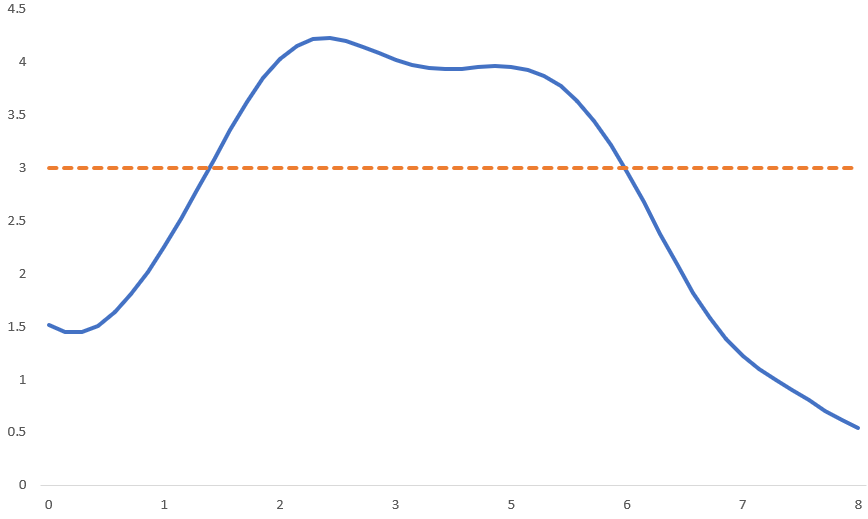
\includegraphics[scale=0.3]{gp_1}
\centering
\caption{Example of a $1d$ gaussian process. The orange line is the mean.}
\label{fig:gp_1} %\ref{fig:gp_1}
\end{figure}

Figure \ref{fig:gp_1} shows a $1d$ gaussian process for uniformly separated $50$ points in the range $[0,8]$. RBF kernel is used with $l = 1$. The values along the $y$ axis are sampled from a normal distribution with mean $3$ and covariance matrix as defined earlier. Note that the normal distribution is defined on a $50$ dimensional space. The mean vector is also $50$ dimensional and the covariance matrix is of shape $50 \times 50$. Any vector sampled from this space will be of size $50$.

%%%%%%%%%%%%%%%%%%%%%%%%%%%%%%%%%%%%%%%%%%%%%%%%%%%%%%%%%%%%%%%%%%%%%%%%%%%
\subsection{Prediction}
For any new point $x \in \mathbb{R}^{d}$, we first assume that $f(x)$ has a prior mean of $0$. Using the Bayes rule,
\begin{align*}
    p(f(x) | f(x_{1}), \ldots, f(x_{N})) &= \frac{p(f(x),f(x_{1}), \ldots, f(x_{N}))}{p(f(x_{1}), \ldots, f(x_{N}))}\\
    &= \frac{\mathcal{N}((0,f(x_{1}),\ldots,f(x_{N})),\tilde{C})}{\mathcal{N}((f(x_{1}),\ldots,f(x_{N})), C)}\\
    C &= \begin{bmatrix} K(0) &K(x_{1} - x_{2}) &\cdots &K(x_{1} - x_{N})\\ \vdots &\vdots &\vdots\\ K(x_{N} - x_{1}) &K(x_{N} - x_{2}) &\cdots &K(0)\\ \end{bmatrix}\\
    \tilde{C} &= \begin{bmatrix} K(0) &k^{T}\\ k &C \end{bmatrix}\\
    k^{T} &= (K(x - x_{1}), K(x - x_{2}), \ldots, K(x - x_{N}))\\
    f^{T} &= (f(x_{1}, f(x_{2}), \ldots, f(x_{N}))
\end{align*}
the ratio of two normals is also a normal distribution, making the final distribution
\begin{align*}
    p(f(x) | f(x_{1}), \ldots, f(x_{N})) = \mathcal{N}(k^{T}C^{-1}f, K(0) - k^{T}C^{-1}k)
\end{align*}

\begin{figure}[h]
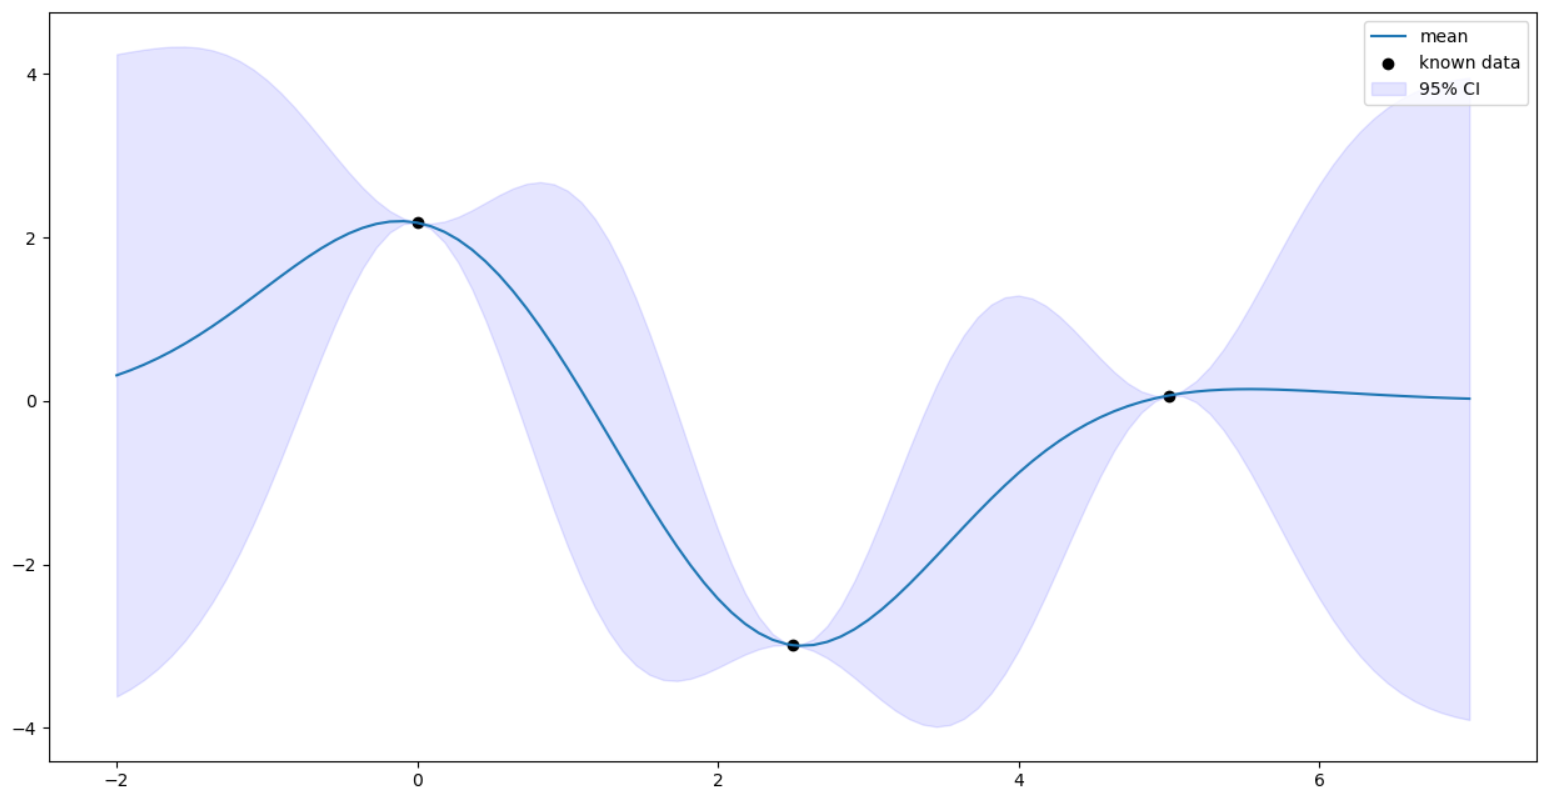
\includegraphics[scale=0.3]{gp_2}
\centering
\caption{Prediction using gaussian process for a $1d$ distribution. Variance of the prediction is $0$ at the observed points. The variance is constant far away from the observed points as $K(0)$ is predefined and finite. Prepared using $gaussian_process_prediction.py$}
\label{fig:gp_2} %\ref{fig:gp_2}
\end{figure}


%%%%%%%%%%%%%%%%%%%%%%%%%%%%%%%%%%%%%%%%%%%%%%%%%%%%%%%%%%%%%%%%%%%%%%%%%%%
\subsubsection*{Prediction with noisy data}
Suppose we observe the points with some noise. If this fact is not taken into account, the gaussian process is sure to overfit the data since it assumes the uncertaininty at observed points to be zero. This will create a very wiggly curve. To counter this, we introduce noise into our kernel itself. The noise is assumed to be independent across samples
\begin{align*}
    \tilde{K}(x1- x2) = K(x1 - x2) + s^{2}I(x1 = x2)
\end{align*}
where $s^{2}$ is the variance of noise $\sim \mathcal{N}(0, s^{2})$.\newline

We have introduced an additional parameter into our model. Suppose we use the RBF kernel. Then we have $\sigma^{2}$ and $l$ as the model parameters also. We can optimize for all of those instead of trying out various values by maximizing the (log)likelihood of the data
\begin{align*}
    \max_{s^{2}, \sigma^{2}, l} p(f(x_{1}, \ldots, x_{n})|s^{2}, \sigma^{2}, l)
    = \max{s^{2}, \sigma^{2}, l} \mathcal{N}(0, \tilde{K})
\end{align*}
which can be done using a method like gradient descent. We can also use only a subset of the data to do the training (similar to SVM where few points near the boundary define it). This leads up to a significant reduction in the run time.


%%%%%%%%%%%%%%%%%%%%%%%%%%%%%%%%%%%%%%%%%%%%%%%%%%%%%%%%%%%%%%%%%%%%%%%%%%%
\subsubsection*{Classification}
Our y in classification is just two labels $\{-1,1 \}$. We assume a latent process $f$
\begin{align*}
    p(y=1|f) &= \frac{1}{1 + exp(-f)}\\
    p^{*}(f(x)) &= p(f(x) | y_{1}(x_{1}, \ldots, y_{N}(x_{N}))\\
    prediction &= \int p(y|f(x))p^{*}(f(x)) d(f(x))
\end{align*}
where we first train to obtain the latent process $f$ which is converted to a probability using the sigmoid function.
\end{document}
